\documentclass{beamer}
%
\mode<presentation>
{
  \usetheme{fnbCD}
}

\usepackage[german]{babel}
\usepackage[latin1]{inputenc}
\usepackage{times}
\usepackage[T1]{fontenc}
\usepackage{multimedia}
\usepackage{hyperref}

\usepackage{mathdesign}
\usepackage[]{subfigure}
\usepackage{float}
\usepackage[]{graphicx}
%\usepackage[]{natbib}
\usepackage[]{amsmath}
\usepackage{dsfont}
\usepackage{color}
%Zur Darstellung von Code
%\usepackage[ruled,chapter]{algorithm}
\usepackage[]{algorithmic}
% Private Declarations
%\usepackage{psfrag}
\usepackage{multirow}
\usepackage{pgfplots}
\pgfplotsset{compat=newest}
\usepackage{tikz}
\usepackage{tikz-3dplot}
\usetikzlibrary{shapes,positioning,calc,arrows.meta,decorations.markings}
\usepackage{tkz-euclide} % loads  TikZ and tkz-base
\usetkzobj{angles} % important you want to use angles
%\usepackage{latexsym}
%\usepackage{pstricks,pst-node}
%\usepackage{pst-blur}
%\usepackage{pstricks-add}
%Colors
%\definecolor{Pink}{rgb}{1.,0.75,0.8}
%\definecolor{fond}{RGB}{240,240,240}
%F�r Bibliography
\usepackage[fixlanguage]{babelbib}
\selectbiblanguage{german}
%\selectlanguage{german}
\usepackage{booktabs}
\usepackage{pgfplots}
\usepackage{rotating}
\usepackage{setspace} %to use \doublespacing in tables
\usepackage{multirow} %multiple rows in tabular environments
\usepackage{booktabs} %provides extra tables commands and in general makes tables look a little nicer than without
\usepackage{colortbl} 
\usepackage{xcolor}   %are required to allow the colour of table and text elements to be altered
\usepackage{xfrac}    %is required to make nicer fractions that look good in tables
\newcommand{\ra}[1]{\renewcommand{\arraystretch}{#1}}
%\usepackage{longtable,tabu,booktabs}
\setbeamercolor{caption name}{fg=fnbblue}
\setbeamerfont{caption name}{size=\tiny}
\setbeamerfont{caption}{size=\tiny}
\setbeamercolor{bibliography entry author}{fg=fnbblue}
\setbeamercolor{bibliography entry journal}{fg=fnbblue}

\title[Masterthesis ]{\small{Implementierung und Untersuchung \\einer hoch effizienten Methode \\zur Druck-Geschwindigkeits-Kopplung}}
\subtitle{\small{Masterthesis}}
%\subtitle
%{- Eine Einf�hrung -}

% usage: \author[short author]{author1\inst{1} \and \author2\inst{2}}
%
%        \institute[short institute]
%        {
%          \inst{1}
%             institute1
%          \and
%          \inst{2}
%             institute2
%        }
%
% short author/short institute necessary only for many authors,
% because optionally go to footer line
%
\author[Fabian Gabel ]{Fabian Gabel}

\institute[FNB, TU Darmstadt]
%{Fachgebiet f�r Numerische Berechnungsverfahren im Maschinenbau\\
%Technische Universit�t Darmstadt}

\date[\today]
{Kolloquium, XX.XX.2015}


\subject{seminar presentation}

% \AtBeginSubsection[]
% {
%   \begin{frame}<beamer>
%     \frametitle{Overview}
%     \tableofcontents[currentsection,currentsubsection]
%   \end{frame}
% }

\pgfdeclareimage[width=\paperwidth]{bg_alt_title}{fnbbeamer-bg-folie4x3-titel-foto-etch}
\pgfdeclareimage[width=\paperwidth]{bg_title}{fnbbeamer-bg-folie4x3-titel-etch}


\begin{document}
%%%%%%%%%%%%%%%%%%%%%%%%%%%%%%%%%%%%%%%%%%%%%%%%%%
% Title page
%%%%%%%%%%%%%%%%%%%%%%%%%%%%%%%%%%%%%%%%%%%%%%%%%%
% 
% usage: \fnbtitlepage{footerright}{alignment}{backgroundimage}

% standard title page is /fnbtitlepage which uses a different 
% backround image, puts the department url in left left bottom 
% corner and some other things.
%

%\fnbtitlepageintro{bg_alt_title}
\fnbtitlepage{\today}{bg_title}
%\fnbtitlepage{\today}{bg_alt_title}

% if you dont want the fnb-titlepage uncomment the following and
% comment out the \fnbtitlepage{}
%
%\begin{frame}
%   \titlepage
%\end{frame}

% choose navigation symbol appearance
% - [only frame symbol]
% - [vertical]
% - [horizontal]
% - {}    (empty hides nav symbols)

\setbeamertemplate{navigation symbols}[only frame symbol]

% placement redefinition because of FNB-Logo
\setbeamertemplate{sidebar right}[fnb theme]

% choose footer
 \setbeamertemplate{footline}[fnb theme]
% \setbeamertemplate{footline}[fnb theme noslidenumber]
% \setbeamertemplate{footline}[fnb theme simplefoot]
% \setbeamertemplate{footline}[fnb theme customfoot]{33}
% \setbeamertemplate{footline}[fnb theme customsimplefoot]{33}

 \begin{frame}
   \frametitle{Inhalt}

% % use
% % \tableofcontents[pausesections]
% % if you want to uncover the sections separately

   %\tableofcontents[pausesections]
   \tableofcontents
 \end{frame}


 \AtBeginSection[]
 {
 \begin{frame}<beamer>
   \frametitle{Inhalt}
     \tableofcontents[currentsection,currentsubsection]
     %\tableofcontents[pausesections]
   \end{frame}
 }

% %
% % Finally, observe to divide your talk in sections and subsections
% % on the one hand this ensures the correct entries in the table of
% % contents and on the other hand the presentation will be easier to 
% % transfer to other styles
% %
% %

% %%%%%%%%%%%%%%%%%%%%%%%%%%%%%%%%%%%%%%%%%%%%%%%%%%%
% %%%%%%%%%%%%%%%%%%%%%%%%%%%%%%%%%%%%%%%%%%%%%%%%%%%
% %%                                               %%
% %%  --- end of setup ---                         %%
% %%                                               %%
% %%%%%%%%%%%%%%%%%%%%%%%%%%%%%%%%%%%%%%%%%%%%%%%%%%%
% %%%%%%%%%%%%%%%%%%%%%%%%%%%%%%%%%%%%%%%%%%%%%%%%%%%

%%%%%%%%%%%%%%%%%%%%%%%%%%%%%%%%%%%%%%%%%%%%%%%%%%%%%%%%%%%%
\section{Motivation}
\begin{frame}

\frametitle{Motivation}
    \vspace{0.5cm}
    Herausforderungen f�r CFD-Applikationen:
    \begin{itemize}
    \item \small{Schnelle Verf�gbarkeit von Simulationsergebnissen}
    \item \small{Ergebnisse mit hoher Genauigkeit}
    \end{itemize}

    \begin{columns}
        \begin{column}{6cm}
            \begin{figure}
            \centering
            \includegraphics[width= 0.8\linewidth]{./img/turbine.jpg}
            \caption{Gasturbine (VDI)}
            \end{figure}
        \end{column}
        \begin{column}{6cm}
            \begin{itemize}
                \item \small{Einsatz robuster Algorithmen}
                \item \small{Skalierbarkeit der L�sungsmethode}
                \item \small{Effizienzsteigerung durch Adaptivit�t}
            \end{itemize}
        \end{column}
    \end{columns}

\end{frame}
%%%%%%%%%%%%%%%%%%%%%%%%%%%%%%%%%%%%%%%%%%%%%%%%%%%%%%%%%%%%
\begin{frame}

\frametitle{Motivation}
    Vollst�ndig gekoppelter L�sungsansatz f�r Navier-Stokes Gleichungen (Darwish 2009):
    \begin{itemize}
    \item Semi-implizite Druck-Geschwindigkeits Kopplung statt sequentieller L�sung
    \item Robuster Algorithmus ohne Unterrelaxation
    \end{itemize}

    \vspace{1cm}
    Neue Herausforderung:
    \begin{itemize}
      \item Umgang mit Speicheranforderungen
      \item Auswahl geeigneter skalierbarer Gleichungsl�ser
    \end{itemize}

\end{frame}
%%%%%%%%%%%%%%%%%%%%%%%%%%%%%%%%%%%%%%%%%%%%%%%%%%%%%%%%%%%%
\section{Aufgabenstellung und Bearbeitung}
\begin{frame}

\frametitle{Aufgabenstellung und Bearbeitung}
  \begin{itemize}
    \item Implementierung eines vollst�ndig gekoppelten L�sungsansatzes 
      \begin{itemize}\scriptsize
        \item Finite-Volumen Diskretisierung der 3d Navier-Stokes Gleichungen auf block-strukturierten, lokal verfeinerten Gittern mit h�ngenden Knoten
        \item Kopplungsans�tze f�r Temperaturgleichung 
        \item MPI-Parallelisierung des L�sungsansatzes mit PETSc
      \end{itemize}
    \item Skalierbarkeitsuntersuchung auf HHLR
    \item Performancevergleich mit herk�mmlichem SIMPLE Verfahren f�r unterschiedliche Testf�lle
      \begin{itemize}\scriptsize
        \item Manufactured Solution
        \item Kanalstr�mung mit komplexem Hindernis
        \item Str�mung in beheizter Kavit�t (Adaption MIT - Benchmark)
      \end{itemize}
  \end{itemize}

\end{frame}
%%%%%%%%%%%%%%%%%%%%%%%%%%%%%%%%%%%%%%%%%%%%%%%%%%%%%%%%%%%%
\section{Implementierung}
\begin{frame}
  \frametitle{Implementierung - Diskretisierung}
\end{frame}
%%%%%%%%%%%%%%%%%%%%%%%%%%%%%%%%%%%%%%%%%%%%%%%%%%%%%%%%%%%%
\begin{frame}
  \frametitle{Implementierung - Temperaturkopplung}
\end{frame}
%%%%%%%%%%%%%%%%%%%%%%%%%%%%%%%%%%%%%%%%%%%%%%%%%%%%%%%%%%%%
\begin{frame}
  \frametitle{Implementierung - Blockr�nder und Parallelisierung}
  Behandlung der Blockr�nder nach Lilek et. al
\end{frame}
%%%%%%%%%%%%%%%%%%%%%%%%%%%%%%%%%%%%%%%%%%%%%%%%%%%%%%%%%%%%
\begin{frame}
\frametitle{Implementierung - Assemblierung}
\begin{columns}
  \begin{column}{0.5cm}
  \end{column}
  \begin{column}{3cm}
  \begin{figure}
    \centering
    \resizebox{1.5\linewidth}{!}{\begin{tikzpicture}
	\coordinate (P1) at (-25cm,6.5cm); % left vanishing point (To pick)
	\coordinate (P2) at (18cm,5.5cm); % right vanishing point (To pick)

	\coordinate (A1) at (0em,0cm); % central top point (To pick)
	\coordinate (A2) at (0em,1.5cm); % central bottom point (To pick)
	\coordinate (A3) at (0em,3cm); % central bottom point (To pick)

	\coordinate (A4) at ($(P1)!.94!(A1)$); 
	\coordinate (A5) at ($(P1)!.94!(A2)$);
	\coordinate (A6) at ($(P1)!.94!(A3)$);

	\coordinate (A7) at ($(P1)!.88!(A1)$); 
	\coordinate (A8) at ($(P1)!.88!(A2)$);
	\coordinate (A9) at ($(P1)!.88!(A3)$);

	\coordinate (A10) at ($(P2)!.94!(A1)$); 
	\coordinate (A11) at ($(P2)!.94!(A2)$);
	\coordinate (A12) at ($(P2)!.94!(A3)$);

	\coordinate (A19) at ($(P2)!.88!(A1)$); 
	\coordinate (A20) at ($(P2)!.88!(A2)$);
	\coordinate (A21) at ($(P2)!.88!(A3)$);

	\coordinate (A13) at
	  (intersection cs: first line={(A10) -- (P1)},
			    second line={(A4) -- (P2)});
	\coordinate (A14) at
	  (intersection cs: first line={(A11) -- (P1)}, 
			    second line={(A5) -- (P2)});
	\coordinate (A15) at
	  (intersection cs: first line={(A12) -- (P1)}, 
			    second line={(A6) -- (P2)});

	\coordinate (A16) at
	  (intersection cs: first line={(A10) -- (P1)},
			    second line={(A7) -- (P2)});
	\coordinate (A17) at
	  (intersection cs: first line={(A11) -- (P1)}, 
			    second line={(A8) -- (P2)});
	\coordinate (A18) at
	  (intersection cs: first line={(A12) -- (P1)}, 
			    second line={(A9) -- (P2)});

	\coordinate (A22) at
	  (intersection cs: first line={(A19) -- (P1)},
			    second line={(A4) -- (P2)});
	\coordinate (A23) at
	  (intersection cs: first line={(A20) -- (P1)}, 
			    second line={(A5) -- (P2)});
	\coordinate (A24) at
	  (intersection cs: first line={(A21) -- (P1)}, 
			    second line={(A6) -- (P2)});

	\coordinate (A25) at
	  (intersection cs: first line={(A19) -- (P1)},
			    second line={(A7) -- (P2)});
	\coordinate (A26) at
	  (intersection cs: first line={(A20) -- (P1)}, 
			    second line={(A8) -- (P2)});
	\coordinate (A27) at
	  (intersection cs: first line={(A21) -- (P1)}, 
			    second line={(A9) -- (P2)});

        \foreach \i in {1,2,3,4,5,6,7,8,9,
                        10,11,12,15,18,
                        19,20,21,24,27}
        {
	 %\draw[fill=black] (A\i) circle (0.15em) ;
        }

        %Vertical Lines
        \draw (A1) -- (A2) -- (A3);
        \draw (A4) -- (A5) -- (A6) -- (A15) -- (A24);
        \draw (A7) -- (A8) -- (A9) -- (A18) -- (A27);
        \draw (A12) -- (A15) -- (A18);
        \draw (A21) -- (A24) -- (A27);

        \fill[gray!30] (A1) -- (A19) -- (A21) -- (A3) -- cycle;
        %Horizontal Lines
        \draw (A7) -- (A4) -- (A1);
        \draw (A8) -- (A5) -- (A2);
        \draw (A9) -- (A6) -- (A3) -- (A12) -- (A21);
        \draw[gray,dashed] (A2) -- (A20);
        \draw[gray,dashed] (A10) -- (A12);
        \draw[gray,dashed] (A1) -- (A19);
        \draw[gray,dashed] (A19) -- (A21);

        %Boundary

	\coordinate (B1) at (0em,0cm);
	\coordinate (B2) at (0em,1cm);
	\coordinate (B3) at (0em,2cm);
	\coordinate (B4) at (0em,3cm);

	\coordinate (B5) at ($(P1)!1.05!(B1)$); 
	\coordinate (B6) at ($(P1)!1.05!(B2)$);
	\coordinate (B7) at ($(P1)!1.05!(B3)$);
	\coordinate (B8) at ($(P1)!1.05!(B4)$);

	\coordinate (B9)  at ($(P1)!1.1!(B1)$); 
	\coordinate (B10) at ($(P1)!1.1!(B2)$);
	\coordinate (B11) at ($(P1)!1.1!(B3)$);
	\coordinate (B12) at ($(P1)!1.1!(B4)$);

	\coordinate (B13)  at ($(P1)!1.15!(B1)$); 
	\coordinate (B14) at ($(P1)!1.15!(B2)$);
	\coordinate (B15) at ($(P1)!1.15!(B3)$);
	\coordinate (B16) at ($(P1)!1.15!(B4)$);

	\coordinate (B17) at ($(P2)!0.96!(B1)$); 
	\coordinate (B18) at ($(P2)!0.96!(B2)$);
	\coordinate (B19) at ($(P2)!0.96!(B3)$);
	\coordinate (B20) at ($(P2)!0.96!(B4)$);

        \coordinate (B33) at ($(P2)!.92!(B1)$); 
        \coordinate (B34) at ($(P2)!.92!(B2)$);
        \coordinate (B35) at ($(P2)!.92!(B3)$);
        \coordinate (B36) at ($(P2)!.92!(B4)$);

        \coordinate (B49) at ($(P2)!.88!(B1)$); 
        \coordinate (B50) at ($(P2)!.88!(B2)$);
        \coordinate (B51) at ($(P2)!.88!(B3)$);
        \coordinate (B52) at ($(P2)!.88!(B4)$);

	\coordinate (B21) at
	  (intersection cs: first line={(B17) -- (P1)},
			    second line={(B5) -- (P2)});
	\coordinate (B22) at
	  (intersection cs: first line={(B18) -- (P1)},
			    second line={(B6) -- (P2)});
	\coordinate (B23) at
	  (intersection cs: first line={(B19) -- (P1)},
			    second line={(B7) -- (P2)});
	\coordinate (B24) at
	  (intersection cs: first line={(B20) -- (P1)},
			    second line={(B8) -- (P2)});

	\coordinate (B25) at
	  (intersection cs: first line={(B17) -- (P1)},
			    second line={(B9) -- (P2)});
	\coordinate (B26) at
	  (intersection cs: first line={(B18) -- (P1)},
			    second line={(B10) -- (P2)});
	\coordinate (B27) at
	  (intersection cs: first line={(B19) -- (P1)},
			    second line={(B11) -- (P2)});
	\coordinate (B28) at
	  (intersection cs: first line={(B20) -- (P1)},
			    second line={(B12) -- (P2)});

	\coordinate (B29) at
	  (intersection cs: first line={(B17) -- (P1)},
			    second line={(B13) -- (P2)});
	\coordinate (B30) at
	  (intersection cs: first line={(B18) -- (P1)},
			    second line={(B14) -- (P2)});
	\coordinate (B31) at
	  (intersection cs: first line={(B19) -- (P1)},
			    second line={(B15) -- (P2)});
	\coordinate (B32) at
	  (intersection cs: first line={(B20) -- (P1)},
			    second line={(B16) -- (P2)});

	\coordinate (B37) at
	  (intersection cs: first line={(B33) -- (P1)},
			    second line={(B5) -- (P2)});
	\coordinate (B38) at
	  (intersection cs: first line={(B34) -- (P1)},
			    second line={(B6) -- (P2)});
	\coordinate (B39) at
	  (intersection cs: first line={(B35) -- (P1)},
			    second line={(B7) -- (P2)});
	\coordinate (B40) at
	  (intersection cs: first line={(B36) -- (P1)},
			    second line={(B8) -- (P2)});

	\coordinate (B41) at
	  (intersection cs: first line={(B33) -- (P1)},
			    second line={(B9) -- (P2)});
	\coordinate (B42) at
	  (intersection cs: first line={(B34) -- (P1)},
			    second line={(B10) -- (P2)});
	\coordinate (B43) at
	  (intersection cs: first line={(B35) -- (P1)},
			    second line={(B11) -- (P2)});
	\coordinate (B44) at
	  (intersection cs: first line={(B36) -- (P1)},
			    second line={(B12) -- (P2)});

	\coordinate (B45) at
	  (intersection cs: first line={(B33) -- (P1)},
			    second line={(B13) -- (P2)});
	\coordinate (B46) at
	  (intersection cs: first line={(B34) -- (P1)},
			    second line={(B14) -- (P2)});
	\coordinate (B47) at
	  (intersection cs: first line={(B35) -- (P1)},
			    second line={(B15) -- (P2)});
	\coordinate (B48) at
	  (intersection cs: first line={(B36) -- (P1)},
			    second line={(B16) -- (P2)});

	\coordinate (B53) at
	  (intersection cs: first line={(B49) -- (P1)},
			    second line={(B5) -- (P2)});
	\coordinate (B54) at
	  (intersection cs: first line={(B50) -- (P1)},
			    second line={(B6) -- (P2)});
	\coordinate (B55) at
	  (intersection cs: first line={(B51) -- (P1)},
			    second line={(B7) -- (P2)});
	\coordinate (B56) at
	  (intersection cs: first line={(B52) -- (P1)},
			    second line={(B8) -- (P2)});

	\coordinate (B57) at
	  (intersection cs: first line={(B49) -- (P1)},
			    second line={(B9) -- (P2)});
	\coordinate (B58) at
	  (intersection cs: first line={(B50) -- (P1)},
			    second line={(B10) -- (P2)});
	\coordinate (B59) at
	  (intersection cs: first line={(B51) -- (P1)},
			    second line={(B11) -- (P2)});
	\coordinate (B60) at
	  (intersection cs: first line={(B52) -- (P1)},
			    second line={(B12) -- (P2)});

	\coordinate (B61) at
	  (intersection cs: first line={(B49) -- (P1)},
			    second line={(B13) -- (P2)});
	\coordinate (B62) at
	  (intersection cs: first line={(B50) -- (P1)},
			    second line={(B14) -- (P2)});
	\coordinate (B63) at
	  (intersection cs: first line={(B51) -- (P1)},
			    second line={(B15) -- (P2)});
	\coordinate (B64) at
	  (intersection cs: first line={(B52) -- (P1)},
			    second line={(B16) -- (P2)});


        %Front lines
        \draw (B13) -- (B29) -- (B45) -- (B61);
        \draw (B1) -- (B5) -- (B9) -- (B13);
        \draw (B2) -- (B6) -- (B10) -- (B14);
        \draw (B3) -- (B7);
        \draw (B14) -- (B62);

        %Vertical lines
        \draw (B5) -- (B6) -- (B7) -- (B8);
        \draw (B29) -- (B30);
        \draw (B45) -- (B46) -- (B47) -- (B48);
        \draw (B61) -- (B62) -- (B63) -- (B64);
        \draw (B13) -- (B14);
        \draw (B9) -- (B10);
        \draw (B38) -- (B40);
        \draw (B22) -- (B24);
        \draw (B42) -- (B44);

        %horizontal lines
        \draw (B22) -- (B26) -- (B30);

        %linien in die tiefe
        \draw (B6) -- (B22); 
        \draw (B7) -- (B39);
        \draw (B10) -- (B42);
        \draw (B47) -- (B63);
        \draw (B48) -- (B64);
        \draw (B44) -- (B60);

        \draw (B8) -- (B24) -- (B40) -- (B56);

        %Top lines (to east)
        \draw (B4) -- (B8);
        \draw (B20) -- (B24);
        \draw (B36) -- (B40) -- (B44) -- (B48);
        \draw (B52) -- (B56) -- (B60) -- (B64);
        \draw (B38) -- (B46);
        \draw (B39) -- (B47);

        %fill out one CV
        \fill[gray!30] (B42) -- (B43) -- (B39) -- (B38) -- cycle;  %back
        \fill[gray!50] (B22) -- (B38) -- (B39) -- (B23) -- cycle;  %left
        \fill[gray!50,opacity=0.2] (B26) -- (B27) -- (B23) -- (B22) -- cycle;  %front
%       \fill[gray!50,opacity=0.7] (B26) -- (B42) -- (B43) -- (B27) -- cycle;  %right
        \fill[gray!90] (B22) -- (B26) -- (B42) -- (B38) -- cycle;  %bottom
        \fill[gray!90,opacity=0.2] (B23) -- (B27) -- (B43) -- (B39) -- cycle;  %top

        \draw[gray!90,dashed] (B8) -- (B16) -- (B48);
        \draw[gray!90,dashed] (B16) -- (B14);
        \draw[gray!90,dashed] (B32) -- (B30);
        \draw[gray!90,dashed] (B12) -- (B10);
        \draw[gray!90,dashed] (B32) -- (B30);
        \draw[gray!90,dashed] (B7) -- (B15) -- (B47);
        \draw[gray!90,dashed] (B23) -- (B31);
        \draw[gray!90,dashed] (B12) -- (B44);
        \draw[gray!90,dashed] (B26) -- (B28);
        \draw[gray!90,dashed] (B24) -- (B32);
        \draw[gray!90,dashed] (B11) -- (B43);

        \draw[gray!90,dashed] (B17) -- (B20);
        \draw[gray!90,dashed] (B33) -- (B36);
        \draw[gray!90,dashed] (B2) -- (B50);
        \draw[gray!90,dashed] (B3) -- (B51);
        \draw[gray!30,dashed] (B49) -- (B61);

        %right lines (vertical)




        \foreach \i in {1,2,3,4,5,6,7,8,9,10,11,12,13,14,15,16,17,18,19,20,21,22,23,24,25,26,27,28,29,30,31,32,33,34,35,36,37,38,39,40,41,42,43,44,45,46,47,48,49,50,51,52,53,54,55,56,57,58,59,60,61,62,63,64}
        {
	 %\draw[fill=black] (B\i) circle (0.15em) ;
        }
        

\end{tikzpicture}
}
    \caption{\tiny{Blockstruturiertes Gitter und resultierende Matrixbelegung f�r eine Variable ohne Kopplung}}
  \end{figure}
  \end{column}
  \begin{column}{10cm}
  \begin{figure}
    \centering
    \label{fig:segassemble}
    \resizebox{.6\linewidth}{!}{
\newcommand*{\xMin}{0}%
\newcommand*{\xMax}{12}%
\newcommand*{\xStep}{0.47}%
\newcommand*{\nStep}{35}
\newcommand*{\yMin}{0}%
\newcommand*{\yMax}{1}%
\newcommand\markcell[3] {
  \fill[gray,draw=black] (#2*\xStep,\xStep*\nStep-#1*\xStep) -- (#2*\xStep+\xStep,\xStep*\nStep-#1*\xStep) -- (#2*\xStep+\xStep,\xStep*\nStep-#1*\xStep-\xStep) -- (#2*\xStep,\xStep*\nStep-#1*\xStep-\xStep) -- cycle;
  \node[anchor=center] at (#2*\xStep+0.5*\xStep,\xStep*\nStep-#1*\xStep-0.5*\xStep) {#3};
  }

\newcommand\markcellblue[3] {
  \fill[orange,draw=black] (#2*\xStep,\xStep*\nStep-#1*\xStep) -- (#2*\xStep+\xStep,\xStep*\nStep-#1*\xStep) -- (#2*\xStep+\xStep,\xStep*\nStep-#1*\xStep-\xStep) -- (#2*\xStep,\xStep*\nStep-#1*\xStep-\xStep) -- cycle;
  \node[anchor=center] at (#2*\xStep+0.5*\xStep,\xStep*\nStep-#1*\xStep-0.5*\xStep) {#3};
  }

\begin{tikzpicture}

    %BACKGROUND COLORING
    \fill[gray!40] (0,\xStep*\nStep-8*\xStep) -- (8*\xStep,\xStep*\nStep-8*\xStep) -- (8*\xStep,0) -- (0*\xStep,0) -- cycle;
    \fill[gray!40] (8*\xStep,\xStep*\nStep) -- (35*\xStep,\xStep*\nStep) -- (35*\xStep,\xStep*\nStep-8*\xStep) -- (8*\xStep,\xStep*\nStep-8*\xStep) -- cycle;

    \foreach \j in {0,...,35} {
        \draw [very thin,gray] (0,\j*\xStep) -- (\xStep*\nStep,\j*\xStep)  ;
        \draw [very thin,gray] (\j*\xStep,0) -- (\j*\xStep,\xStep*\nStep)  ;
    }

    \foreach \j in {0,...,34} {
        \node[anchor=center] at (-0.3,\xStep*\nStep-\j*\xStep-0.5*\xStep) {\j};
        \node[anchor=center] at (\j*\xStep+0.5*\xStep,\xStep*\nStep+0.3) {\j};
    }

    \foreach \i in {0,...,34} {
      \markcell {\i}{\i}{$a_P$};
    }

    %BLOCK 1
    \markcell {0}{1}{$a_N$};
    \markcell {0}{2}{$a_E$};
    \markcell {0}{4}{$a_T$};

    \markcell {1}{0}{$a_S$};
    \markcell {1}{3}{$a_E$};
    \markcell {1}{5}{$a_T$};

    \markcell {2}{3}{$a_N$};
    \markcell {2}{0}{$a_W$};
    \markcell {2}{6}{$a_T$};

    \markcell {3}{2}{$a_S$};
    \markcell {3}{1}{$a_W$};
    \markcell {3}{7}{$a_T$};

    \markcell {4}{5}{$a_N$};
    \markcell {4}{6}{$a_E$};
    \markcell {4}{0}{$a_B$};

    \markcell {5}{4}{$a_S$};
    \markcell {5}{7}{$a_E$};
    \markcell {5}{1}{$a_B$};

    \markcell {6}{7}{$a_N$};
    \markcell {6}{4}{$a_W$};
    \markcell {6}{2}{$a_B$};

    \markcell {7}{6}{$a_S$};
    \markcell {7}{5}{$a_W$};
    \markcell {7}{3}{$a_B$};
     
    %BLOCK2
    \markcell {8 }{9 }{$a_N$};
    \markcell {8 }{11}{$a_E$};
    \markcell {8 }{17}{$a_T$};

    \markcell {9 }{8 }{$a_S$};
    \markcell {9 }{10}{$a_N$};
    \markcell {9 }{12}{$a_E$};
    \markcell {9 }{18}{$a_T$};

    \markcell {10}{9 }{$a_S$};
    \markcell {10}{13}{$a_E$};
    \markcell {10}{19}{$a_T$};

    \markcell {11}{8 }{$a_W$};
    \markcell {11}{12}{$a_N$};
    \markcell {11}{14}{$a_E$};
    \markcell {11}{20}{$a_T$};

    \markcell {12 }{9 }{$a_W$};
    \markcell {12 }{11}{$a_S$};
    \markcell {12 }{13}{$a_N$};
    \markcell {12 }{15}{$a_E$};
    \markcell {12 }{21}{$a_T$};

    \markcell {13}{10}{$a_W$};
    \markcell {13}{12}{$a_S$};
    \markcell {13}{16}{$a_E$};
    \markcell {13}{22}{$a_T$};

    \markcell {14}{11}{$a_W$};
    \markcell {14}{15}{$a_N$};
    \markcell {14}{23}{$a_T$};

    \markcell {15 }{12}{$a_W$};
    \markcell {15 }{14}{$a_S$};
    \markcell {15 }{16}{$a_N$};
    \markcell {15 }{24}{$a_T$};

    \markcell {16}{13}{$a_W$};
    \markcell {16}{15}{$a_S$};
    \markcell {16}{25}{$a_T$};



    \markcell {17 }{18 }{$a_N$};
    \markcell {17 }{20}{$a_E$};
    \markcell {17 }{26}{$a_T$};
    \markcell {17}{8 }{$a_B$};

    \markcell {18 }{17 }{$a_S$};
    \markcell {18 }{19}{$a_N$};
    \markcell {18 }{21}{$a_E$};
    \markcell {18 }{27}{$a_T$};
    \markcell {18}{9 }{$a_B$};

    \markcell {19}{18 }{$a_S$};
    \markcell {19}{22}{$a_E$};
    \markcell {19}{28}{$a_T$};
    \markcell {19}{10}{$a_B$};

    \markcell {20}{17}{$a_W$};
    \markcell {20}{21}{$a_N$};
    \markcell {20}{23}{$a_E$};
    \markcell {20}{29}{$a_T$};
    \markcell {20}{11}{$a_B$};

    \markcell {21}{18 }{$a_W$};
    \markcell {21}{20}{$a_S$};
    \markcell {21}{22}{$a_N$};
    \markcell {21}{24}{$a_E$};
    \markcell {21}{30}{$a_T$};
    \markcell {21}{12}{$a_B$};

    \markcell {22}{19}{$a_W$};
    \markcell {22}{21}{$a_S$};
    \markcell {22}{25}{$a_E$};
    \markcell {22}{31}{$a_T$};
    \markcell {22}{13}{$a_B$};

    \markcell {23}{20}{$a_W$};
    \markcell {23}{24}{$a_N$};
    \markcell {23}{32}{$a_T$};
    \markcell {23}{14}{$a_B$};

    \markcell {24}{21}{$a_W$};
    \markcell {24}{23}{$a_S$};
    \markcell {24}{25}{$a_N$};
    \markcell {24}{33}{$a_T$};
    \markcell {24}{15}{$a_B$};

    \markcell {25}{22}{$a_W$};
    \markcell {25}{24}{$a_S$};
    \markcell {25}{34}{$a_T$};
    \markcell {25}{16}{$a_B$};



    \markcell {26}{27}{$a_N$};
    \markcell {26}{29}{$a_E$};
    \markcell {26}{17}{$a_B$};

    \markcell {27}{26}{$a_S$};
    \markcell {27}{28}{$a_N$};
    \markcell {27}{30}{$a_E$};
    \markcell {27}{18}{$a_B$};

    \markcell {28}{27}{$a_S$};
    \markcell {28}{31}{$a_E$};
    \markcell {28}{19}{$a_B$};

    \markcell {29}{26}{$a_W$};
    \markcell {29}{30}{$a_N$};
    \markcell {29}{32}{$a_E$};
    \markcell {29}{20}{$a_B$};

    \markcell {30}{27}{$a_W$};
    \markcell {30}{29}{$a_S$};
    \markcell {30}{31}{$a_N$};
    \markcell {30}{33}{$a_E$};
    \markcell {30}{21}{$a_B$};

    \markcell {31}{28}{$a_W$};
    \markcell {31}{30}{$a_S$};
    \markcell {31}{34}{$a_E$};
    \markcell {31}{22}{$a_B$};

    \markcell {32}{29}{$a_W$};
    \markcell {32}{33}{$a_N$};
    \markcell {32}{23}{$a_B$};

    \markcell {33}{30}{$a_W$};
    \markcell {33}{32}{$a_S$};
    \markcell {33}{34}{$a_N$};
    \markcell {33}{24}{$a_B$};

    \markcell {34}{31}{$a_W$};
    \markcell {34}{33}{$a_S$};
    \markcell {34}{25}{$a_B$};

    %Connectivities
    \markcellblue {2}{8}{$a_R$};
    \markcellblue {2}{9}{$a_R$};
    \markcellblue {2}{17}{$a_R$};
    \markcellblue {2}{18}{$a_R$};

    \markcellblue {3}{9}{$a_R$};
    \markcellblue {3}{10}{$a_R$};
    \markcellblue {3}{18}{$a_R$};
    \markcellblue {3}{19}{$a_R$};

    \markcellblue {6}{17}{$a_R$};
    \markcellblue {6}{18}{$a_R$};
    \markcellblue {6}{26}{$a_R$};
    \markcellblue {6}{27}{$a_R$};

    \markcellblue {7}{18}{$a_R$};
    \markcellblue {7}{19}{$a_R$};
    \markcellblue {7}{27}{$a_R$};
    \markcellblue {7}{28}{$a_R$};

    \markcellblue {8}{2}{$a_L$};
    \markcellblue {9}{2}{$a_L$};
    \markcellblue {17}{2}{$a_L$};
    \markcellblue {18}{2}{$a_L$};

    \markcellblue {9}{3}{$a_L$};
    \markcellblue {10}{3}{$a_L$};
    \markcellblue {18}{3}{$a_L$};
    \markcellblue {19}{3}{$a_L$};

    \markcellblue {17}{6}{$a_L$};
    \markcellblue {18}{6}{$a_L$};
    \markcellblue {26}{6}{$a_L$};
    \markcellblue {27}{6}{$a_L$};

    \markcellblue {18}{7}{$a_L$};
    \markcellblue {19}{7}{$a_L$};
    \markcellblue {27}{7}{$a_L$};
    \markcellblue {28}{7}{$a_L$};

    \draw[ultra thick] (0,\xStep*\nStep) -- (8*\xStep,\xStep*\nStep) -- (8*\xStep,\xStep*\nStep-8*\xStep) -- (0,\xStep*\nStep-8*\xStep) -- cycle;
    \draw[ultra thick] (8*\xStep,\xStep*\nStep) -- (35*\xStep,\xStep*\nStep) -- (35*\xStep,\xStep*\nStep-8*\xStep) -- (8*\xStep,\xStep*\nStep-8*\xStep) -- cycle;
    \draw[ultra thick] (8*\xStep,\xStep*\nStep-8*\xStep) -- (35*\xStep,\xStep*\nStep-8*\xStep) -- (35*\xStep,0) -- (8*\xStep,0) -- cycle;
    \draw[ultra thick] (0,\xStep*\nStep-8*\xStep) -- (8*\xStep,\xStep*\nStep-8*\xStep) -- (8*\xStep,0) -- (0*\xStep,0) -- cycle;

\end{tikzpicture}
}
%\caption{Non-zero structure of the linear systems used in the SIMPLE algorithm for a block-structured grid consisting of one  $2\times2\times2$ cell and one $3\times3\times3$ cell block}
  \end{figure}
  \end{column}
\end{columns}
\end{frame}
%%%%%%%%%%%%%%%%%%%%%%%%%%%%%%%%%%%%%%%%%%%%%%%%%%%%%%%%%%%%
\begin{frame}
\frametitle{Implementierung - Assemblierung mit Kopplung}
\vspace{-0.5cm}
\begin{columns}
\begin{column}{7cm}
\begin{figure}
  \centering
  \label{fig:cpldassemble}
  \resizebox{\linewidth}{!}{
\newcommand*{\xMin}{0}%
\newcommand*{\xMax}{12}%
\newcommand*{\xStep}{1.5}%
\newcommand*{\nStep}{5}
\newcommand*{\yMin}{0}%
\newcommand*{\yMax}{1}%
\newcommand\markcell[3] {
  \fill[gray,draw=black] (#2*\xStep,\xStep*\nStep-#1*\xStep) -- (#2*\xStep+\xStep,\xStep*\nStep-#1*\xStep) -- (#2*\xStep+\xStep,\xStep*\nStep-#1*\xStep-\xStep) -- (#2*\xStep,\xStep*\nStep-#1*\xStep-\xStep) -- cycle;
  \node[anchor=center,font=\large] at (#2*\xStep+0.5*\xStep,\xStep*\nStep-#1*\xStep-0.5*\xStep) {#3};
  }

\newcommand\markcellblue[3] {
  \fill[cyan,draw=black] (#2*\xStep,\xStep*\nStep-#1*\xStep) -- (#2*\xStep+\xStep,\xStep*\nStep-#1*\xStep) -- (#2*\xStep+\xStep,\xStep*\nStep-#1*\xStep-\xStep) -- (#2*\xStep,\xStep*\nStep-#1*\xStep-\xStep) -- cycle;
  \node[anchor=center,font=\large] at (#2*\xStep+0.5*\xStep,\xStep*\nStep-#1*\xStep-0.5*\xStep) {#3};
  }

\newcommand\markcellred[3] {
  \fill[red,draw=black] (#2*\xStep,\xStep*\nStep-#1*\xStep) -- (#2*\xStep+\xStep,\xStep*\nStep-#1*\xStep) -- (#2*\xStep+\xStep,\xStep*\nStep-#1*\xStep-\xStep) -- (#2*\xStep,\xStep*\nStep-#1*\xStep-\xStep) -- cycle;
  \node[anchor=center,font=\large] at (#2*\xStep+0.5*\xStep,\xStep*\nStep-#1*\xStep-0.5*\xStep) {#3};
  }

\newcommand\markcellgreen[3] {
  \fill[green,draw=black] (#2*\xStep,\xStep*\nStep-#1*\xStep) -- (#2*\xStep+\xStep,\xStep*\nStep-#1*\xStep) -- (#2*\xStep+\xStep,\xStep*\nStep-#1*\xStep-\xStep) -- (#2*\xStep,\xStep*\nStep-#1*\xStep-\xStep) -- cycle;
  \node[anchor=center,font=\large] at (#2*\xStep+0.5*\xStep,\xStep*\nStep-#1*\xStep-0.5*\xStep) {#3};
  }

\newcommand*{\xStepp}{0.15}%
\newcommand*{\nStepp}{35}
\newcommand*{\offset}{5}
\newcommand\markcelll[3] {
  \fill[gray,draw=black] (#2*\xStepp-\offset,\xStepp*\nStepp-#1*\xStepp-\offset) -- (#2*\xStepp+\xStepp-\offset,\xStepp*\nStepp-#1*\xStepp-\offset) -- (#2*\xStepp+\xStepp-\offset,\xStepp*\nStepp-#1*\xStepp-\xStepp-\offset) -- (#2*\xStepp-\offset,\xStepp*\nStepp-#1*\xStepp-\xStepp-\offset) -- cycle;
  }

\newcommand\markcellbluee[3] {
  \fill[orange,draw=black] (#2*\xStepp-\offset,\xStepp*\nStepp-#1*\xStepp-\offset) -- (#2*\xStepp+\xStepp-\offset,\xStepp*\nStepp-#1*\xStepp-\offset) -- (#2*\xStepp+\xStepp-\offset,\xStepp*\nStepp-#1*\xStepp-\xStepp-\offset) -- (#2*\xStepp-\offset,\xStepp*\nStepp-#1*\xStepp-\xStepp-\offset) -- cycle;
  }

\newcommand\markcellblackk[3] {
  \fill[black,draw=black] (#2*\xStepp-\offset,\xStepp*\nStepp-#1*\xStepp-\offset) -- (#2*\xStepp+\xStepp-\offset,\xStepp*\nStepp-#1*\xStepp-\offset) -- (#2*\xStepp+\xStepp-\offset,\xStepp*\nStepp-#1*\xStepp-\xStepp-\offset) -- (#2*\xStepp-\offset,\xStepp*\nStepp-#1*\xStepp-\xStepp-\offset) -- cycle;
  }

\begin{tikzpicture}


    %SMALL MATRIX%%%%%%%%%%%%%%%%%%%%%%%%%%%%%%%%%%%%%%%%%%%%%%%%%%%%%%%%%%%%%%%%%%%%%%%%%%%%%%%%%%%%%%%%%%%%%%%%%%%%%%%%%%%%%%%%%%
    %BACKGROUND COLORING
    \fill[gray!40] (0-\offset,\xStepp*\nStepp-8*\xStepp-\offset) -- (8*\xStepp-\offset,\xStepp*\nStepp-8*\xStepp-\offset) -- (8*\xStepp-\offset,0-\offset) -- (0*\xStepp-\offset,0-\offset) -- cycle;
    \fill[gray!40] (8*\xStepp-\offset,\xStepp*\nStepp-\offset) -- (35*\xStepp-\offset,\xStepp*\nStepp-\offset) -- (35*\xStepp-\offset,\xStepp*\nStepp-\offset-8*\xStepp) -- (8*\xStepp-\offset,\xStepp*\nStepp-8*\xStepp-\offset) -- cycle;

    \foreach \j in {0,...,35} {
        \draw [very thin,gray] (0-\offset,\j*\xStepp-\offset) -- (\xStepp*\nStepp-\offset,\j*\xStepp-\offset)  ;
        \draw [very thin,gray] (\j*\xStepp-\offset,0-\offset) -- (\j*\xStepp-\offset,\xStepp*\nStepp-\offset)  ;
    }

    \foreach \i in {0,...,34} {
      \markcelll {\i}{\i}{};
    }

    %BLOCK 1
    \markcelll {0}{1}{};
    \markcelll {0}{2}{};
    \markcelll {0}{4}{};

    \markcelll {1}{0}{};
    \markcelll {1}{3}{};
    \markcelll {1}{5}{};

    \markcelll {2}{3}{};
    \markcelll {2}{0}{};
    \markcelll {2}{6}{};

    \markcelll {3}{2}{};
    \markcelll {3}{1}{};
    \markcelll {3}{7}{};

    \markcelll {4}{5}{};
    \markcelll {4}{6}{};
    \markcelll {4}{0}{};

    \markcelll {5}{4}{};
    \markcelll {5}{7}{};
    \markcelll {5}{1}{};

    \markcelll {6}{7}{};
    \markcelll {6}{4}{};
    \markcelll {6}{2}{};

    \markcelll {7}{6}{};
    \markcelll {7}{5}{};
    \markcelll {7}{3}{};
     
    %BLOCK2
    \markcelll {8 }{9 }{};
    \markcelll {8 }{11}{};
    \markcelll {8 }{17}{};

    \markcelll {9 }{8 }{};
    \markcelll {9 }{10}{};
    \markcelll {9 }{12}{};
    \markcelll {9 }{18}{};

    \markcelll {10}{9 }{};
    \markcelll {10}{13}{};
    \markcelll {10}{19}{};

    \markcelll {11}{8 }{};
    \markcelll {11}{12}{};
    \markcelll {11}{14}{};
    \markcelll {11}{20}{};

    \markcelll {12 }{9 }{};
    \markcelll {12 }{11}{};
    \markcelll {12 }{13}{};
    \markcelll {12 }{15}{};
    \markcelll {12 }{21}{};

    \markcelll {13}{10}{};
    \markcelll {13}{12}{};
    \markcelll {13}{16}{};
    \markcelll {13}{22}{};

    \markcelll {14}{11}{};
    \markcelll {14}{15}{};
    \markcelll {14}{23}{};

    \markcelll {15 }{12}{};
    \markcelll {15 }{14}{};
    \markcelll {15 }{16}{};
    \markcelll {15 }{24}{};

    \markcelll {16}{13}{};
    \markcelll {16}{15}{};
    \markcelll {16}{25}{};

    \markcelll {17}{18 }{};
    \markcelll {17}{20}{};
    \markcelll {17}{26}{};
    \markcelll {17}{8 }{};

    \markcelll {18}{17}{};
    \markcelll {18}{19}{};
    \markcelll {18}{21}{};
    \markcelll {18}{27}{};
    \markcelll {18}{9 }{};

    \markcelll {19}{18}{};
    \markcelll {19}{22}{};
    \markcelll {19}{28}{};
    \markcelll {19}{10}{};

    \markcelll {20}{17}{};
    \markcelll {20}{21}{};
    \markcelll {20}{23}{};
    \markcelll {20}{29}{};
    \markcelll {20}{11}{};

    \markcelll {21}{18}{};
    \markcelll {21}{20}{};
    \markcelll {21}{22}{};
    \markcelll {21}{24}{};
    \markcelll {21}{30}{};
    \markcelll {21}{12}{};

    \markcelll {22}{19}{};
    \markcelll {22}{21}{};
    \markcelll {22}{25}{};
    \markcelll {22}{31}{};
    \markcelll {22}{13}{};

    \markcelll {23}{20}{};
    \markcelll {23}{24}{};
    \markcelll {23}{32}{};
    \markcelll {23}{14}{};

    \markcelll {24}{21}{};
    \markcelll {24}{23}{};
    \markcelll {24}{25}{};
    \markcelll {24}{33}{};
    \markcelll {24}{15}{};

    \markcelll {25}{22}{};
    \markcelll {25}{24}{};
    \markcelll {25}{34}{};
    \markcelll {25}{16}{};



    \markcelll {26}{27}{};
    \markcelll {26}{29}{};
    \markcelll {26}{17}{};

    \markcelll {27}{26}{};
    \markcelll {27}{28}{};
    \markcelll {27}{30}{};
    \markcelll {27}{18}{};

    \markcelll {28}{27}{};
    \markcelll {28}{31}{};
    \markcelll {28}{19}{};

    \markcelll {29}{26}{};
    \markcelll {29}{30}{};
    \markcelll {29}{32}{};
    \markcelll {29}{20}{};

    \markcelll {30}{27}{};
    \markcelll {30}{29}{};
    \markcelll {30}{31}{};
    \markcelll {30}{33}{};
    \markcelll {30}{21}{};

    \markcelll {31}{28}{};
    \markcelll {31}{30}{};
    \markcelll {31}{34}{};
    \markcelll {31}{22}{};

    \markcelll {32}{29}{};
    \markcelll {32}{33}{};
    \markcelll {32}{23}{};

    \markcelll {33}{30}{};
    \markcelll {33}{32}{};
    \markcelll {33}{34}{};
    \markcelll {33}{24}{};

    \markcelll {34}{31}{};
    \markcelll {34}{33}{};
    \markcelll {34}{25}{};

    %Connectivities
    \markcellbluee {2}{8}{};
    \markcellbluee {2}{9}{};
    \markcellbluee {2}{17}{};
    \markcellbluee {2}{18}{};

    \markcellbluee {3}{9}{};
    \markcellbluee {3}{10}{};
    \markcellbluee {3}{18}{};
    \markcellbluee {3}{19}{};

    \markcellbluee {6}{17}{};
    \markcellbluee {6}{18}{};
    \markcellbluee {6}{26}{};
    \markcellbluee {6}{27}{};

    \markcellbluee {7}{18}{};
    \markcellbluee {7}{19}{};
    \markcellbluee {7}{27}{};
    \markcellbluee {7}{28}{};

    \markcellbluee {8}{2}{};
    \markcellbluee {9}{2}{};
    \markcellbluee {17}{2}{};
    \markcellbluee {18}{2}{};

    \markcellbluee {9}{3}{};
    \markcellbluee {10}{3}{};
    \markcellbluee {18}{3}{};
    \markcellbluee {19}{3}{};

    \markcellbluee {17}{6}{};
    \markcellbluee {18}{6}{};
    \markcellbluee {26}{6}{};
    \markcellbluee {27}{6}{};

    \markcellbluee {18}{7}{};
    \markcellbluee {19}{7}{};
    \markcellbluee {27}{7}{};
    \markcellbluee {28}{7}{};

    \draw[ultra thick] (0-\offset,\xStepp*\nStepp-\offset) -- (8*\xStepp-\offset,\xStepp*\nStepp-\offset) -- (8*\xStepp-\offset,\xStepp*\nStepp-8*\xStepp-\offset) -- (0-\offset,\xStepp*\nStepp-8*\xStepp-\offset) -- cycle;
    \draw[ultra thick] (8*\xStepp-\offset,\xStepp*\nStepp-\offset) -- (35*\xStepp-\offset,\xStepp*\nStepp-\offset) -- (35*\xStepp-\offset,\xStepp*\nStepp-8*\xStepp-\offset) -- (8*\xStepp-\offset,\xStepp*\nStepp-8*\xStepp-\offset) -- cycle;
    \draw[ultra thick] (8*\xStepp-\offset,\xStepp*\nStepp-8*\xStepp-\offset) -- (35*\xStepp-\offset,\xStepp*\nStepp-8*\xStepp-\offset) -- (35*\xStepp-\offset,0-\offset) -- (8*\xStepp-\offset,0-\offset) -- cycle;
    \draw[ultra thick] (0-\offset,\xStepp*\nStepp-8*\xStepp-\offset) -- (8*\xStepp-\offset,\xStepp*\nStepp-8*\xStepp-\offset) -- (8*\xStepp-\offset,0-\offset) -- (0*\xStepp-\offset,0-\offset) -- cycle;

    \coordinate (A1) at (21*\xStepp-\offset,\xStepp*\nStepp-21*\xStepp-\offset);
    \coordinate (A2) at (21*\xStepp+\xStepp-\offset,\xStepp*\nStepp-21*\xStepp-\offset);
    \coordinate (A3) at (21*\xStepp+\xStepp-\offset,\xStepp*\nStepp-21*\xStepp-\xStepp-\offset);
    \coordinate (A4) at (21*\xStepp-\offset,\xStepp*\nStepp-21*\xStepp-\xStepp-\offset);
    \markcellblackk {21}{21}{};

    %\draw[fill=black] (A1) circle (0.15em);
    %\draw[fill=black] (A2) circle (0.15em);
    %\draw[fill=black] (A3) circle (0.15em);
    %\draw[fill=black] (A4) circle (0.15em);

    \draw[ultra thick] (A1) -- (0,7.5);
    \draw[ultra thick] (A2) -- (7.5,7.5);
    \draw[ultra thick] (A3) -- (7.5,0);
    \draw[ultra thick] (A4) -- (0,0);

    %CPLD MATRIX%%%%%%%%%%%%%%%%%%%%%%%%%%%%%%%%%%%%%%%%%%%%%%%%%%%%%%%%%%%%%%%%%%%%%%%%%%%%%%%%%%%%%%%%%%%%%%%%%%%%%%%%%%%%%%%%%%
    \foreach \j in {0,...,5} {
        \draw [very thin,gray] (0,\j*\xStep) -- (\xStep*\nStep,\j*\xStep)  ;
        \draw [very thin,gray] (\j*\xStep,0) -- (\j*\xStep,\xStep*\nStep)  ;
    }

    \markcell {0}{0}{$a_P^{u_1}$};
    \markcell {1}{1}{$a_P^{u_2}$};
    \markcell {2}{2}{$a_P^{u_3}$};
    \markcell {3}{3}{$a_P^{p}$};
    \markcell {4}{4}{$a_P^{T}$};

    \markcellblue{0}{3}{$a_P^{u_1,p}$};
    \markcellblue{1}{3}{$a_P^{u_2,p}$};
    \markcellblue{2}{3}{$a_P^{u_3,p}$};

    \markcellblue{3}{0}{$a_P^{p,u_1}$};
    \markcellblue{3}{1}{$a_P^{p,u_2}$};
    \markcellblue{3}{2}{$a_P^{p,u_3}$};

    \markcellred{0}{4}{$a_P^{u_1,T}$};
    \markcellred{1}{4}{$a_P^{u_2,T}$};
    \markcellred{2}{4}{$a_P^{u_3,T}$};

    \markcellgreen{4}{0}{$a_P^{T,u_1}$};
    \markcellgreen{4}{1}{$a_P^{T,u_2}$};
    \markcellgreen{4}{2}{$a_P^{T,u_3}$};
    \markcellgreen{4}{3}{$a_P^{T,p}$};

   \draw[ultra thick] (0,\xStep*\nStep) -- (4*\xStep,\xStep*\nStep) -- (4*\xStep,\xStep*\nStep-4*\xStep) -- (0,\xStep*\nStep-4*\xStep) -- cycle;
   \draw[ultra thick] (4*\xStep,\xStep*\nStep) -- (5*\xStep,\xStep*\nStep) -- (5*\xStep,\xStep*\nStep-3*\xStep) -- (4*\xStep,\xStep*\nStep-3*\xStep) -- cycle;
   \draw[ultra thick] (0,\xStep*\nStep) -- (5*\xStep,\xStep*\nStep) -- (5*\xStep,\xStep*\nStep-5*\xStep) -- (0,\xStep*\nStep-5*\xStep) -- cycle;
   \draw[ultra thick] (0,\xStep*\nStep-4*\xStep) -- (4*\xStep,\xStep*\nStep-4*\xStep) -- (4*\xStep,\xStep*\nStep-5*\xStep) -- (0,\xStep*\nStep-5*\xStep) -- cycle;


\end{tikzpicture}
}
  %\caption{Matrixstruktur f�r Blockmatrizen}
\end{figure}
\end{column}
\begin{column}{5cm}
  \begin{itemize}\scriptsize
    \item blau: Druck-Geschwindigkeit
    \item rot: Geschwindkigkeit-Temperatur
    \item gr�n: Temperatur-Geschwindigkeit/Druck
  \end{itemize}
\end{column}
\end{columns}
\end{frame}
%%%%%%%%%%%%%%%%%%%%%%%%%%%%%%%%%%%%%%%%%%%%%%%%%%%%%%%%%%%%
\begin{frame}
  \frametitle{Implementierung - L�sungsalgorithmus}
\end{frame}
%%%%%%%%%%%%%%%%%%%%%%%%%%%%%%%%%%%%%%%%%%%%%%%%%%%%%%%%%%%%
\section{Performanceuntersuchung}
%%%%%%%%%%%%%%%%%%%%%%%%%%%%%%%%%%%%%%%%%%%%%%%%%%%%%%%%%%%%
\begin{frame}
  \frametitle{STREAM Benchmark - Sustainable Memory Bandwidth}
\end{frame}
%%%%%%%%%%%%%%%%%%%%%%%%%%%%%%%%%%%%%%%%%%%%%%%%%%%%%%%%%%%%
\begin{frame}
  \frametitle{Manufactured Solution}
\end{frame}
%%%%%%%%%%%%%%%%%%%%%%%%%%%%%%%%%%%%%%%%%%%%%%%%%%%%%%%%%%%%
\begin{frame}
  \frametitle{Manufactured Solution - Strong-Scaling}
\end{frame}
%%%%%%%%%%%%%%%%%%%%%%%%%%%%%%%%%%%%%%%%%%%%%%%%%%%%%%%%%%%%
\begin{frame}
  \frametitle{Manufactured Solution - Weak-Scaling}
\end{frame}
%%%%%%%%%%%%%%%%%%%%%%%%%%%%%%%%%%%%%%%%%%%%%%%%%%%%%%%%%%%%
\begin{frame}
  \frametitle{Kanalstr�mung - Problemstellung}
\end{frame}
%%%%%%%%%%%%%%%%%%%%%%%%%%%%%%%%%%%%%%%%%%%%%%%%%%%%%%%%%%%%
\begin{frame}
  \frametitle{Kanalstr�mung - Druck-Geschwindigkeitskopplung}
\end{frame}
%%%%%%%%%%%%%%%%%%%%%%%%%%%%%%%%%%%%%%%%%%%%%%%%%%%%%%%%%%%%
\begin{frame}
\frametitle{Beheizte Kavit�t - Problemstellung}
\begin{columns}
  \begin{column}{4cm}
    \begin{figure}[h!]
    \centering
    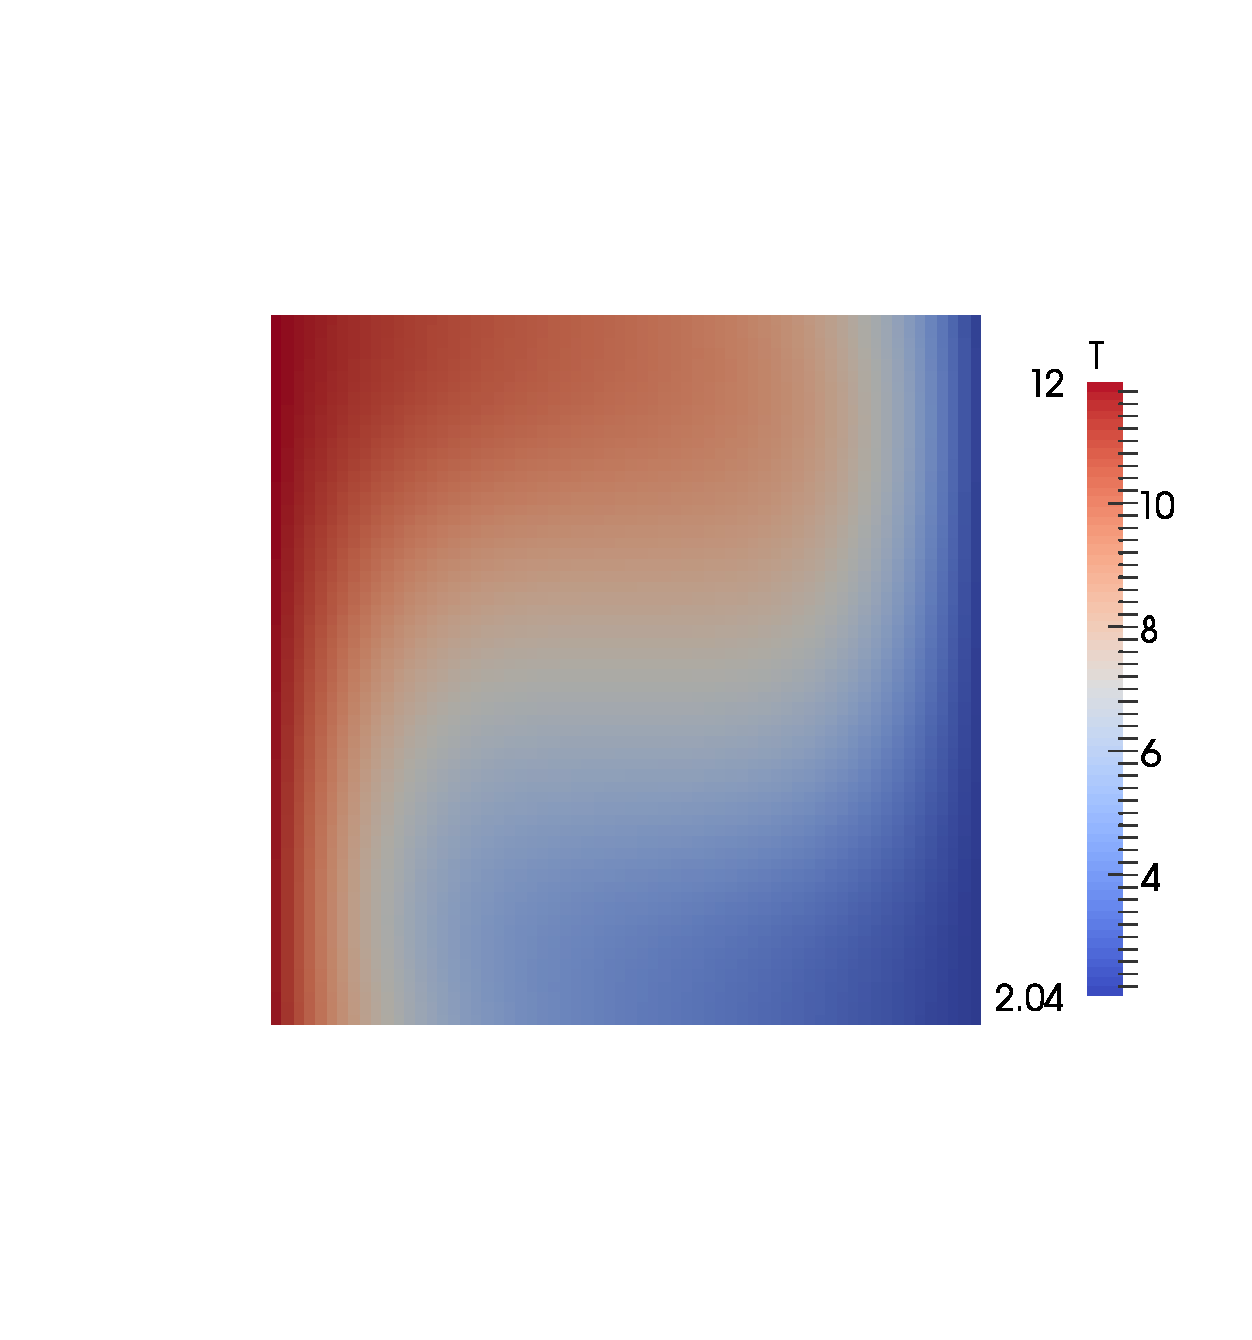
\includegraphics[trim=3.5cm 5cm 0cm 5cm, scale=0.5,clip=true]{./img/cavity.pdf}
    \end{figure}
  \end{column}
 \begin{column}{4cm}
   \begin{figure}[h!]
   \centering
   %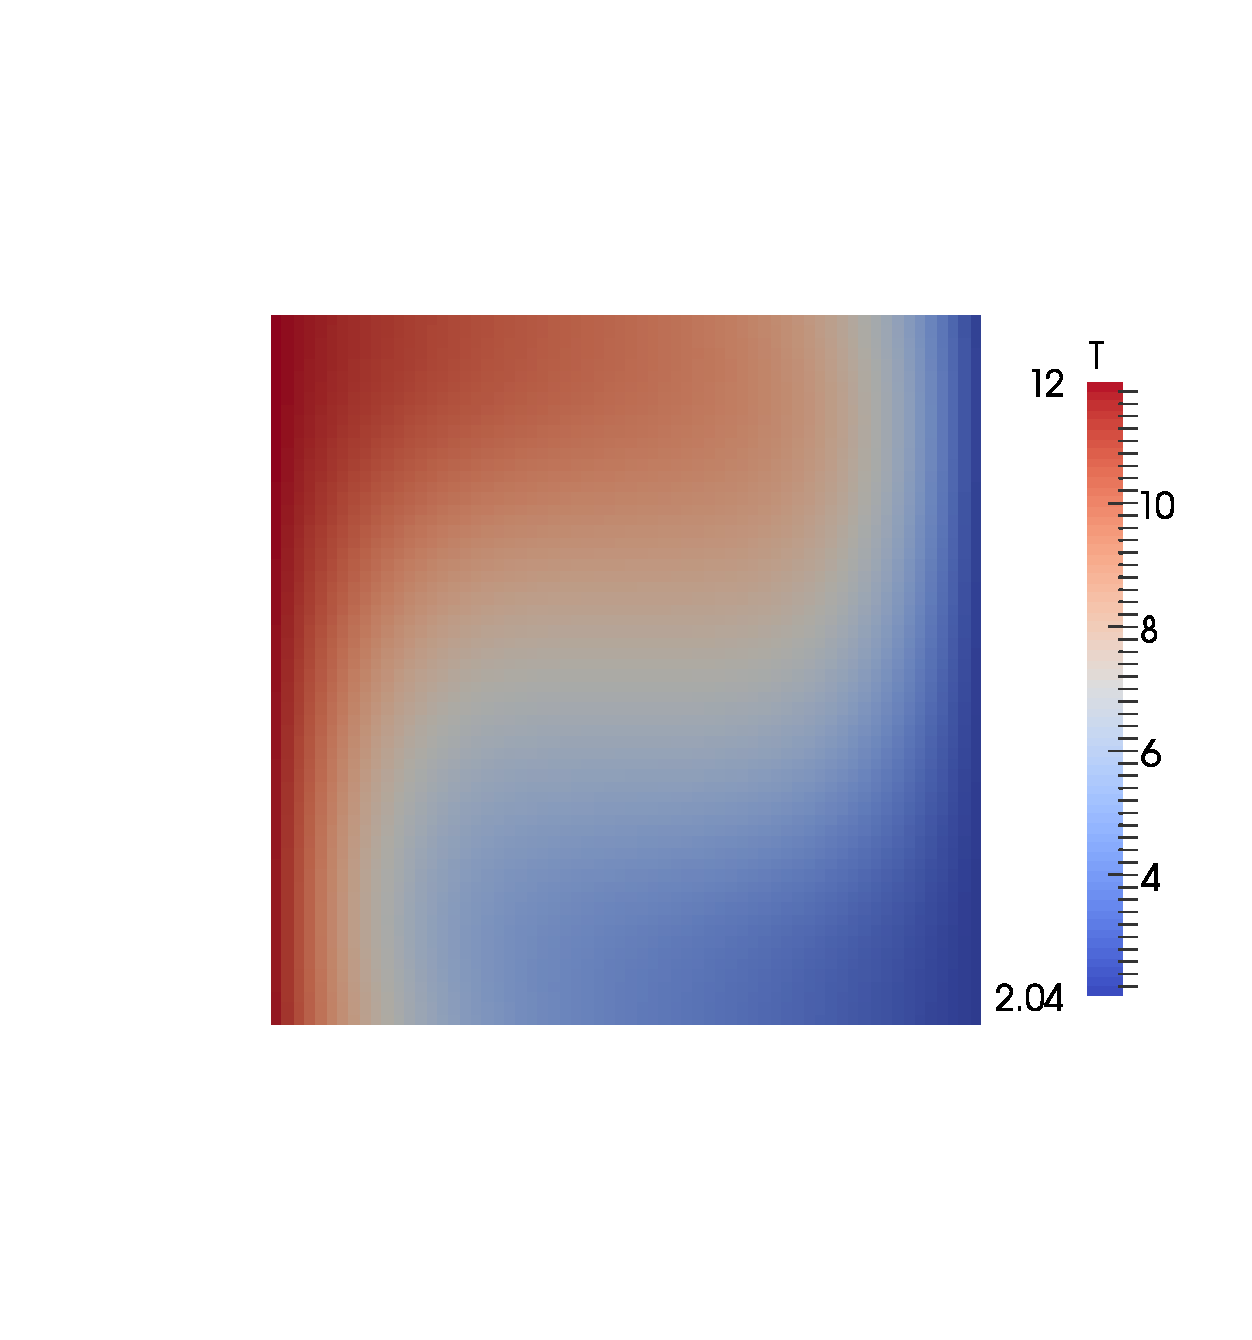
\includegraphics[trim=3.5cm 5cm 0cm 5cm, scale=0.5,clip=true]{./img/cavity.pdf}
   \end{figure}
 \end{column}
\end{columns}
\end{frame}
%%%%%%%%%%%%%%%%%%%%%%%%%%%%%%%%%%%%%%%%%%%%%%%%%%%%%%%%%%%%
\begin{frame}
  \frametitle{Beheizte Kavit�t - Temperaturkopplung}

\begin{table}[h!]\centering
\ra{1.3}
\caption{Performance des SIMPLE algorithmus (SEG), des gekoppelten Algorithmus (CPLD) mit impliziter Boussinesq Approximation (TCPLD) und semi-impliziter Temperatur-Geschwindigkeits/Druck-Kopplung (NRCPLD).}
\resizebox{7cm}{!}{
\begin{tabular}{cccc}\toprule
    Resolution & Solver configuration & Time & No. Non-linear its. \\
    \midrule
    \rowcolor{black!20}\multirow{4}{*}{}            & SEG    & 0.3719E+02 & 203 \\
    \rowcolor{black!20}                             & CPLD   & 0.6861E+02 & 62  \\
    \rowcolor{black!20}                             & TCPLD  & 0.1012E+03 & 31  \\
    \rowcolor{black!20} \multirow{-4}{*}{32x32x32}  & NRCPLD & 0.2153E+02 & 22  \\ %\hline
    %
    \rowcolor{black!00}\multirow{4}{*}{}            & SEG    & 0.1997E+04 &  804 \\
    \rowcolor{black!00}                             & CPLD   & 0.7687E+03 &  63  \\
    \rowcolor{black!00}                             & TCPLD  & 0.1278E+04 &  59  \\
    \rowcolor{black!00} \multirow{-4}{*}{64x64x64}  & NRCPLD & 0.4240E+03 &  17  \\ %\hline
    %
    \rowcolor{black!20}\multirow{4}{*}{}               & SEG    & 0.5197E+05 &  3060 \\
    \rowcolor{black!20}                                & CPLD   & 0.1860E+05 &  74   \\
    \rowcolor{black!20}                                & TCPLD  & 0.1950E+05 &  50   \\
    \rowcolor{black!20} \multirow{-4}{*}{128x128x128}  & NRCPLD & 0.6155E+04 &  18   \\ %\hline
    %
    %\rowcolor{black!00}\multirow{4}{*}{}               & SEG    &  & \\
    %\rowcolor{black!00}                                & CPLD   &  & \\
    %\rowcolor{black!00}                                & TCPLD  &  & \\
    %\rowcolor{black!00} \multirow{-4}{*}{256x256x256}  & NRCPLD &  & \\ %\hline
  \end{tabular}
}
  \label{tab:cavitycompare}
\end{table}

\end{frame}
%%%%%%%%%%%%%%%%%%%%%%%%%%%%%%%%%%%%%%%%%%%%%%%%%%%%%%%%%%%%
\section{Fazit und Ausblick}
\begin{frame}
  \frametitle{Fazit}
\end{frame}
%%%%%%%%%%%%%%%%%%%%%%%%%%%%%%%%%%%%%%%%%%%%%%%%%%%%%%%%%%%%
\begin{frame}
  \frametitle{Ausblick}
\end{frame}
%%%%%%%%%%%%%%%%%%%%%%%%%%%%%%%%%%%%%%%%%%%%%%%%%%%%%%%%%%%%


 
\end{document}




